\section{Problem: Multiplicity}
\label{multiplicity}
\indent
 When a student begins to learn something, he/she
 depends on the abilities of his tutor to choose the 
 material to study for a given course.
 \par
 
 \indent
 Once he has the basic bibliography, he often finds
 that there is multiplicity in the content of the 
 various references, that is, there are topics that
 are addressed in more than one source.
 \par
 
 \indent
 The student is in a dilemma, he usually doesn't
 have the time to read all the references, but he
 may read the one which may not be the most useful 
 or appropiate to his learning style.
 \par
 
 \indent
 The student is then forced to explore the different
 references in order to find which may be the best 
 path of study.
 \par



\paragraph{Studying: Blind exploration of the topics}

\indent
We may imagine he exploration of the references as 
exploring the different branches of a tree, in which 
the nodes represent the key concepts and the links 
the connecting ideas between those concepts.
\par

\indent
In a typical scenario the student is on his own exploring 
different references and each attempt to undertand a concept
may be regarded as a branch in the tree. Since he has a 
buch of references but doesn't really know them this tree 
has multiple branches leading to the same concept, that 
is multiplicity of branches. 
\par

\indent
That's not always a bad thing, if the branches are legit, that
is, they represents mutually exclusive paths to the same concept.
\par

\indent
Unfortunately more often than not the concepts explained in 
different references are the same and there should be a standarized
way to present them. 
\begin{Large}\textbf{(Why?)}\end{Large}.
\par

\begin{figure}[htp]
 \centering
 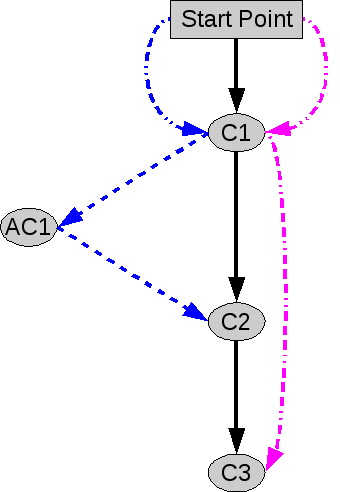
\includegraphics[width=2in]{../img/blind-exploration-tree.png}
 \caption{Blind exploration of ...}
 \label{fig:blind-exploration-tree}
\end{figure}